\documentclass[12pt, a4paper]{article}

% ── Packages ──────────────────────────────────────────────────────────────────
\usepackage[a4paper, margin=2.5cm]{geometry}
\usepackage{graphicx}
\usepackage{float}
\usepackage{amsmath}
\usepackage{amssymb}
\usepackage{xcolor}
\usepackage{mdframed}
\usepackage{parskip}
\usepackage{enumitem}
\usepackage{titlesec}
\usepackage{booktabs}
\usepackage{hyperref}
\usepackage[T1]{fontenc}
\usepackage[colorinlistoftodos]{todonotes}

% ── Graphics path ─────────────────────────────────────────────────────────────
\graphicspath{{../../Images_for_latex/Lecture_2/}}

% ── Colours ───────────────────────────────────────────────────────────────────
\definecolor{keyblue}{RGB}{30, 80, 160}
\definecolor{keybluebg}{RGB}{220, 235, 255}
\definecolor{noteorange}{RGB}{200, 100, 0}
\definecolor{noteorangebg}{RGB}{255, 240, 215}
\definecolor{warnred}{RGB}{180, 30, 30}
\definecolor{warnredbg}{RGB}{255, 220, 220}
\definecolor{defgreen}{RGB}{20, 110, 50}
\definecolor{defgreenbg}{RGB}{215, 245, 225}
\definecolor{headernavy}{RGB}{25, 35, 90}

% ── Box environments ──────────────────────────────────────────────────────────

% Key Takeaway box (blue)
\newmdenv[
  linecolor=keyblue,
  backgroundcolor=keybluebg,
  linewidth=1.5pt,
  leftline=true, rightline=false, topline=false, bottomline=false,
  innerleftmargin=10pt,
  innerrightmargin=8pt,
  innertopmargin=6pt,
  innerbottommargin=6pt,
  skipabove=8pt,
  skipbelow=8pt,
]{keybox}

% Note box (orange)
\newmdenv[
  linecolor=noteorange,
  backgroundcolor=noteorangebg,
  linewidth=1.5pt,
  leftline=true, rightline=false, topline=false, bottomline=false,
  innerleftmargin=10pt,
  innerrightmargin=8pt,
  innertopmargin=6pt,
  innerbottommargin=6pt,
  skipabove=8pt,
  skipbelow=8pt,
]{notebox}

% Warning box (red)
\newmdenv[
  linecolor=warnred,
  backgroundcolor=warnredbg,
  linewidth=1.5pt,
  leftline=true, rightline=false, topline=false, bottomline=false,
  innerleftmargin=10pt,
  innerrightmargin=8pt,
  innertopmargin=6pt,
  innerbottommargin=6pt,
  skipabove=8pt,
  skipbelow=8pt,
]{warnbox}

% Definition box (green)
\newmdenv[
  linecolor=defgreen,
  backgroundcolor=defgreenbg,
  linewidth=1.5pt,
  leftline=true, rightline=false, topline=false, bottomline=false,
  innerleftmargin=10pt,
  innerrightmargin=8pt,
  innertopmargin=6pt,
  innerbottommargin=6pt,
  skipabove=8pt,
  skipbelow=8pt,
]{defbox}

% ── Section formatting ────────────────────────────────────────────────────────
\titleformat{\section}[block]
  {\large\bfseries\color{headernavy}}
  {}
  {0pt}
  {}
  [\vspace{2pt}\rule{\linewidth}{0.8pt}\vspace{4pt}]

\titleformat{\subsection}[block]
  {\normalsize\bfseries\color{keyblue}}
  {}
  {0pt}
  {}

% ── Commands for labels ───────────────────────────────────────────────────────
\newcommand{\keynote}[1]{\textbf{\color{keyblue}#1}}
\newcommand{\warn}[1]{\textbf{\color{warnred}#1}}

% ── Document ──────────────────────────────────────────────────────────────────
\begin{document}
\listoftodos
\clearpage
% ── Title ─────────────────────────────────────────────────────────────────────
\begin{center}
  {\LARGE\bfseries\color{headernavy} Sensors \& Systems}\\[4pt]
  {\large Simple Sensors --- Slides 1--9}\\[2pt]
  {\normalsize Jan Bendtsen, Torben Knudsen \quad|\quad Electronic Systems, 8th Semester}
\end{center}

\vspace{4pt}
\hrule height 1.2pt
\vspace{12pt}

% ==============================================================================
%  TOPIC: What is a Simple Sensor?
% ==============================================================================
\section*{Slides 1--3 \quad What Is a ``Simple'' Sensor?}

The lecture covers: Hall sensor, temperature sensor, humidity sensor,
measurement noise (Gaussian, thermal, flicker, shot), and simple filtering.

\begin{figure}[H]
  \centering
  
\includegraphics[width=0.75\linewidth]{slide-03.jpg}
  \caption{Three ``simple'' sensors: air-quality (left), Hall effect (centre),
           microphone (right).}
  \label{fig:slide03}
\end{figure}

A \textbf{simple sensor} is a self-contained device that converts a single,
continuous physical quantity into an electrical signal with little or no
additional computation required on the user's side.
Three defining properties hold for all simple sensors:

\begin{itemize}[leftmargin=1.5em]
  \item It measures \textbf{one continuous physical quantity} --- temperature,
        magnetic field strength, sound pressure, humidity, etc.
  \item It provides a \textbf{simple interface} --- either an analog voltage/current
        output or a straightforward digital protocol
        (I\textsuperscript{2}C, SPI, UART, etc.).
  \item It does \textbf{not require extensive processing} to obtain the desired
        measurement --- contrast this with a camera or radar, where significant
        computation must precede any useful output.
\end{itemize}

\begin{defbox}
  \textbf{Definition --- Simple Sensor:} a sensor that
  (1)~measures a single continuous physical quantity,
  (2)~provides a simple analog or digital interface, and
  (3)~requires no extensive post-processing to obtain the desired
  information.
\end{defbox}

% ==============================================================================
%  TOPIC: The Sensor Signal Chain
% ==============================================================================
\section*{Slide 4 \quad The Sensor Signal Chain}

\begin{figure}[H]
  \centering
  
\includegraphics[width=0.95\linewidth]{slide-04.jpg}
  \caption{The general sensor signal chain: physical event $\to$ sensing
           component $\to$ amplifier $\to$ ADC $\to$ computing.}
  \label{fig:slide04}
\end{figure}

Every sensor --- simple or otherwise --- follows the same general processing
pipeline from the physical world to a number in your microcontroller.
Understanding this chain is important because it tells you \emph{where} a
particular sensor sits and what processing remains your responsibility.

\begin{enumerate}[leftmargin=1.5em]
  \item \textbf{Physical event.} A real-world phenomenon occurs --- light,
        sound, temperature change, force, radiation. This is the stimulus
        the sensor exists to measure.

  \item \textbf{Sensing component.} A transducer converts the physical
        phenomenon into an electrical signal, typically a voltage or current.
        This is the core physics step. The output is often tiny --- millivolts
        or microamps.

  \item \textbf{Amplifier.} The weak electrical signal is boosted to a level
        suitable for the ADC. Because sensor signals are small, amplifier
        quality matters; any noise or offset introduced here gets amplified
        alongside the signal.

  \item \textbf{Analog-to-Digital Converter (ADC).} The amplified continuous
        signal is sampled at regular intervals $T_s$ and converted to a
        digital integer. This is where the continuous physical world becomes a
        discrete-time sequence of values. Output protocols include
        PWM, RS232, I\textsuperscript{2}C, SPI, and CAN.

  \item \textbf{Computing.} A microcontroller or processor interprets the
        stream of digital values and acts on them.
\end{enumerate}

\begin{notebox}
  \textbf{Note --- integration level.} Different sensors integrate different
  numbers of these stages internally. A bare PT100 resistance thermometer
  gives you only a raw resistance --- stages 2 onward are your problem.
  A TMP117 integrates the amplifier and ADC on-chip and hands you
  temperature in \textdegree{}C directly over I\textsuperscript{2}C.
  Always check the datasheet to know what the sensor does for you.
\end{notebox}

\begin{keybox}
  \textbf{Key Takeaway:} The same five-stage chain governs every sensor
  system. ``Simple'' sensors merely make stages 3--4 (and sometimes 5)
  invisible to the user by integrating them on-chip.
\end{keybox}

% ==============================================================================
%  TOPIC: Hall Effect Sensor
% ==============================================================================
\section*{Slides 5--7 \quad The Hall Effect Sensor}

\subsection*{What Is a Hall Sensor For?}

A Hall sensor is used to \textbf{measure or detect magnetic fields}.
Just as a thermistor converts temperature into a resistance,
a Hall sensor converts magnetic field strength (flux density,
measured in Gauss or Tesla) into a voltage.

Practical uses include:
\begin{itemize}[leftmargin=1.5em]
  \item Detecting the presence of a magnet (e.g.\ reed-switch replacement,
        door/lid open--closed detection).
  \item Measuring rotation speed --- a magnet on a shaft passes the sensor
        once per revolution, producing a pulse.
  \item Measuring current --- a current-carrying conductor generates a
        magnetic field proportional to the current.
  \item Measuring the position of a magnetic actuator or joystick.
\end{itemize}

\subsection*{The Physics of the Hall Effect (Slide 6)}
\todo[inline]{Maybe go back and look at Flux Density and how i think need to be percendicalur to someting} 
\begin{figure}[H]
  \centering
  
\includegraphics[width=0.95\linewidth]{slide-06.jpg}
  \caption{Left: no magnetic field, $V_\mathrm{HALL}\approx 0$\,V.
           Right: magnetic field perpendicular to bias current,
           $V_\mathrm{HALL}$ rises proportionally.}
  \label{fig:slide06}
\end{figure}

Inside the sensor there is a thin \textbf{semiconductor sheet}.
A constant voltage source forces a fixed \textbf{bias current}
$I_\mathrm{BIAS}$ through the sheet along its length.

\begin{itemize}[leftmargin=1.5em]
  \item \textbf{No field:} charge carriers flow straight through the sheet;
        the voltage measured \emph{across the width}, $V_\mathrm{HALL}$,
        is approximately zero.
  \item \textbf{Field present:} flux lines enter the semiconductor
        perpendicular to $I_\mathrm{BIAS}$. The Lorentz force
        $\mathbf{F} = q\mathbf{v} \times \mathbf{B}$ deflects the charge
        carriers sideways, causing charge accumulation along one edge.
        This creates a measurable transverse voltage ---
        $V_\mathrm{HALL}$ rises toward a positive value.
\end{itemize}

The key relationship is:
\[
  V_\mathrm{HALL} \propto I_\mathrm{BIAS} \cdot B
\]
where $B$ is the magnetic flux density. Since $I_\mathrm{BIAS}$ is kept
constant, $V_\mathrm{HALL}$ varies \textbf{linearly} with $B$.

\begin{defbox}
  \textbf{Variable summary:}
  \begin{itemize}[leftmargin=1.5em, topsep=2pt]
    \item $I_\mathrm{BIAS}$ --- constant bias current forced through the
          semiconductor sheet.
    \item $B$ --- magnetic flux density (Gauss / Tesla); the quantity
          being measured.
    \item $V_\mathrm{HALL}$ --- output voltage across the \emph{width}
          of the sheet; $\approx 0$ with no field, proportional to $B$
          when a field is present.
  \end{itemize}
\end{defbox}

\subsection*{Signal Conditioning --- Two Configurations (Slide 7)}

\begin{figure}[H]
  \centering
  
\includegraphics[width=0.95\linewidth]{slide-07.jpg}
  \caption{Left: linear Hall sensor (Hall element + OpAmp only).
           Right: switch-type Hall sensor (Hall element + OpAmp +
           comparator/Schmitt trigger).}
  \label{fig:slide07}
\end{figure}

$V_\mathrm{HALL}$ is typically only a few millivolts --- far too small to
be useful on its own. Two different goals lead to two different circuit
configurations:

\subsubsection*{Configuration 1 --- Measuring Field Strength (linear sensor)}

Connect a precision OpAmp directly after the Hall element.
The OpAmp amplifies $V_\mathrm{HALL}$ to a usable level; the output
is an analog voltage proportional to $B$.

\begin{warnbox}
  \warn{Warning:} this configuration demands a \textbf{high-quality,
  low-offset OpAmp}. Any DC offset is amplified alongside the signal ---
  a 1\,mV offset with a gain of 500 becomes 500\,mV of error,
  completely swamping a small magnetic signal.
\end{warnbox}

\subsubsection*{Configuration 2 --- Detecting Presence Only (switch-type sensor)}

Add a \textbf{comparator (Schmitt trigger)} after the amplifier.
The comparator outputs a clean digital HIGH or LOW based on whether
the amplified $V_\mathrm{HALL}$ exceeds a threshold.

\begin{itemize}[leftmargin=1.5em]
  \item Small OpAmp offsets are absorbed by the comparator threshold ---
        a lower-grade OpAmp is acceptable.
  \item The Schmitt trigger adds \textbf{hysteresis}: turn-on and turn-off
        thresholds differ slightly, preventing chattering near the boundary.
\end{itemize}

\begin{keybox}
  \textbf{Key Takeaway --- choosing a configuration:}
  \begin{itemize}[leftmargin=1.5em, topsep=2pt]
    \item Need a \emph{proportional} measurement of field strength?
          $\to$ Linear Hall sensor (OpAmp only).
          Requires a high-quality OpAmp; output is analog.
    \item Need only \emph{presence/absence} detection?
          $\to$ Switch-type Hall sensor (OpAmp + comparator).
          Tolerates a lower-grade OpAmp; output is digital.
  \end{itemize}
\end{keybox}

% ==============================================================================
%  TOPIC: SS49E Linear Hall Sensor
% ==============================================================================
\section*{Slide 8 \quad The SS49E Linear Hall Sensor}

\begin{figure}[H]
  \centering
  
\includegraphics[width=0.60\linewidth]{slide-08.jpg}
  \caption{The SS49E linear Hall effect sensor module.}
  \label{fig:slide08}
\end{figure}

The SS49E is a specific \textbf{linear} Hall sensor --- it uses
Configuration~1 and provides a continuous analog output
proportional to field strength. Key specifications:

\begin{itemize}[leftmargin=1.5em]
  \item \textbf{Sensitivity: $2.5 \pm 0.5$\,mV/G.}
        For every Gauss of magnetic flux density, the output voltage
        changes by approximately 2.5\,mV. The $\pm 0.5$\,mV/G
        tolerance means unit-to-unit sensitivity variation of up to 20\%
        --- calibration is advisable in precision applications.
  \item \textbf{Power consumption: 4\,mA at 5\,V DC.}
        Modest consumption; compatible with direct Arduino/microcontroller
        supply.
  \item \textbf{Minimum supply: 2.3\,V.}
        The sensor can run from 3.3\,V systems (Raspberry Pi, Nordic MCUs,
        etc.) without a level shifter.
\end{itemize}

\begin{notebox}
  \textbf{Note --- sensitivity tolerance.} The $\pm 0.5$\,mV/G spread
  means two sensors from the same batch may give readings that differ
  by up to 20\% for the same field. For precise measurements, each
  unit should be individually calibrated against a known field.
\end{notebox}

% ==============================================================================
%  TOPIC: Arduino Example
% ==============================================================================
\section*{Slide 9 \quad Arduino Example --- Reading the SS49E}

\begin{figure}[H]
  \centering
  
\includegraphics[width=0.95\linewidth]{slide-09.jpg}
  \caption{Wiring diagram and Arduino code for reading the SS49E.}
  \label{fig:slide09}
\end{figure}

The example code on slide~9 demonstrates a complete reading pipeline.

\subsubsection*{Step 1 --- Averaging to reduce noise}
\begin{verbatim}
long measure = 0;
for(int i = 0; i < 10; i++){
    measure += analogRead(pinHall);
}
measure /= 10;
\end{verbatim}

Ten successive ADC readings are accumulated and divided by 10 ---
a basic \textbf{averaging filter}. Averaging $N$ independent noise
samples reduces the noise standard deviation by a factor of $\sqrt{N}$,
so averaging 10 readings gives $\sqrt{10}\approx 3.2\times$ noise
reduction at the cost of 10 ADC conversions.

\subsubsection*{Step 2 --- ADC count to millivolts}
\begin{verbatim}
float outputV = measure * 5000.0 / 1023;
\end{verbatim}

The Arduino Uno's ADC has \textbf{10-bit resolution}: it maps 0--5\,V
onto integers 0--1023. Multiplying by $5000/1023$ recovers the voltage
in millivolts.

\subsubsection*{Step 3 --- Millivolts to magnetic flux density}
\begin{verbatim}
float magneticFlux = outputV * 53.33 - 133.3;
\end{verbatim}

This is the \textbf{inverse of the sensor's sensitivity curve},
converting millivolts back to flux density in millitesla.
The subtraction of 133.3 accounts for the sensor's quiescent output
at zero field (the output sits at mid-supply when no field is present,
not at 0\,V --- this offset must be removed).

\begin{keybox}
  \textbf{Key Takeaways --- Hall sensor end-to-end:}
  \begin{itemize}[leftmargin=1.5em, topsep=2pt]
    \item A Hall sensor converts \textbf{magnetic field strength} to a
          voltage via the Hall effect.
    \item $V_\mathrm{HALL}$ is tiny; an OpAmp is always needed.
    \item For field \emph{strength} measurements use a linear sensor
          (analog output). For field \emph{presence} detection use a
          switch-type sensor (digital output).
    \item The SS49E has sensitivity $2.5 \pm 0.5$\,mV/G;
          calibration is recommended for precision work.
    \item Averaging multiple ADC readings is a simple and effective
          way to reduce measurement noise --- a preview of the filtering
          concepts covered later in this lecture.
  \end{itemize}
\end{keybox}

% ==============================================================================
%  TOPIC: Temperature Sensor — NTC Thermistor
% ==============================================================================
\clearpage
\section*{Slides 10--11 \quad Temperature Sensor: NTC Thermistor}

A \textbf{Negative Temperature Coefficient (NTC) thermistor} is a resistor
whose resistance \emph{decreases} as temperature increases.
It is one of the most common simple temperature sensors due to its low cost,
wide availability, and large resistance change over temperature.

\subsection*{Voltage Divider Readout (Slide 11)}

\begin{figure}[H]
  \centering
  
\includegraphics[width=0.70\linewidth]{slide-11.jpg}
  \caption{Voltage-divider circuit: $v$ is the supply, $R_\mathrm{meas}$ is
           a fixed reference resistor, and $R_\mathrm{NTC}(\vartheta(t))$
           is the thermistor.}
  \label{fig:slide11}
\end{figure}

The NTC is read out using a simple \textbf{voltage divider}.
A known supply voltage $v$ is applied across the series combination of a
fixed resistor $R_\mathrm{meas}$ and the thermistor $R_\mathrm{NTC}$.
The voltage \emph{across} $R_\mathrm{meas}$ is fed to the ADC --- ``across''
means the ADC is connected at the \textbf{node between the two resistors}
(the positive end of $R_\mathrm{meas}$) and at GND (its negative end).
That node sits between the two components in the chain:

\begin{center}
\ttfamily\small
\begin{tabular}{c}
v (supply)\\
|\\
{[R\_NTC]} \quad $\leftarrow$ thermistor\\
|\\
$\bullet$ \textbf{--- ADC reads here} \quad ($V_\mathrm{out}$ = voltage at this node w.r.t.\ GND)\\
|\\
{[R\_meas]} \quad $\leftarrow$ fixed resistor\\
|\\
GND
\end{tabular}
\end{center}

\[
  V_\mathrm{out} = v \cdot \frac{R_\mathrm{meas}}{R_\mathrm{meas} + R_\mathrm{NTC}(\vartheta)}
\]

Because $R_\mathrm{NTC}$ changes with temperature $\vartheta$, so does
$V_\mathrm{out}$ — the ADC reading can then be converted back to temperature
using the thermistor's characteristic curve from its datasheet.

\begin{notebox}
  \textbf{Note --- choice of $R_\mathrm{meas}$.}
  Sensitivity is highest when $R_\mathrm{meas} \approx R_\mathrm{NTC}$ at
  the centre of your temperature range. Choosing $R_\mathrm{meas}$ equal to
  the thermistor's nominal resistance (e.g.\ 10\,k$\Omega$ at 25\,\textdegree{}C)
  is a common starting point.

  \medskip
  The intuition comes from the two extremes:
  \begin{itemize}[leftmargin=1.5em, topsep=2pt]
    \item $R_\mathrm{meas} \gg R_\mathrm{NTC}$ --- almost all of $v$ drops
          across $R_\mathrm{meas}$ permanently; the thermistor barely
          influences $V_\mathrm{out}$.
    \item $R_\mathrm{meas} \ll R_\mathrm{NTC}$ --- almost all of $v$ drops
          across $R_\mathrm{NTC}$ permanently; $V_\mathrm{out}$ sits near
          zero and barely moves.
    \item $R_\mathrm{meas} = R_\mathrm{NTC}$ --- neither resistor dominates,
          so a small change in $R_\mathrm{NTC}$ shifts the balance the most,
          giving the largest swing in $V_\mathrm{out}$.
  \end{itemize}
\end{notebox}

\begin{keybox}
  \textbf{Key Takeaway:} An NTC thermistor requires only a fixed resistor and
  an ADC to read temperature. The non-linear $R$--$T$ relationship means a
  lookup table or the Steinhart--Hart equation is needed to convert the ADC
  reading to a calibrated temperature.
\end{keybox}

% ==============================================================================
%  TOPIC: Combined Temperature and Humidity Sensor — DHT11
% ==============================================================================
\section*{Slides 12--14 \quad Combined Sensor: DHT11}

\subsection*{Sensor Overview (Slide 12)}

\begin{figure}[H]
  \centering
  
\includegraphics[width=0.65\linewidth]{slide-12.jpg}
  \caption{The DHT11 combined temperature and humidity sensor.}
  \label{fig:slide12}
\end{figure}

The \textbf{DHT11} integrates both a humidity sensor and a temperature sensor
(NTC thermistor) in one package with a single-wire digital interface.
Key specifications:

\begin{itemize}[leftmargin=1.5em]
  \item \textbf{Humidity:} 20\%--80\,\% relative humidity, accuracy $\pm$5\,\%
  \item \textbf{Temperature:} 0\,\textdegree{}C to 50\,\textdegree{}C,
        accuracy $\pm$2\,\textdegree{}C
  \item \textbf{Supply:} 3.0\,V to 5.5\,V; current 0.3\,mA (measuring),
        60\,$\mu$A (idle)
  \item \textbf{Sampling rate:} 1\,Hz maximum
  \item \textbf{Response time:} 6\,s to 15\,s
\end{itemize}

\begin{warnbox}
  \warn{Warning --- slow response time.} The DHT11 can only be sampled at
  1\,Hz, and its thermal and humidity response time is 6--15\,s. It is
  unsuitable for applications that need fast or frequent measurements.

  \medskip
  \textbf{Sampling rate vs.\ response time:}
  \begin{itemize}[leftmargin=1.5em, topsep=2pt]
    \item \textbf{Sampling rate} --- how often you can \emph{ask} for a reading (1\,Hz).
    \item \textbf{Response time} --- how long the physical element takes to
          \emph{react} to a real change (6--15\,s).
  \end{itemize}

  \medskip
  Even sampling at 1\,Hz, a sudden jump in the environment is spread across
  multiple samples --- the output creeps toward the true value rather than
  jumping in one step:

\begin{center}
\ttfamily\small
\begin{tabular}{lrrrrrrr}
True humidity: & 20\% & -- & -- & -- & -- & -- & 80\% \\
DHT11 output:  & 20\% & 25\% & 35\% & 50\% & 65\% & 75\% & 80\% \\
Time:          & 0\,s & 1\,s & 2\,s & 3\,s & 4\,s & 5\,s & 6\,s+ \\
\end{tabular}
\end{center}
\end{warnbox}

\subsection*{How the Humidity Sensor Works (Slide 13)}

\begin{figure}[H]
  \centering
  
\includegraphics[width=0.75\linewidth]{slide-13.jpg}
  \caption{Capacitive humidity sensing principle inside the DHT11.}
  \label{fig:slide13}
\end{figure}

The humidity element is a \textbf{capacitive sensor} with two electrodes
and a moisture-absorbing substrate in between:

\begin{enumerate}[leftmargin=1.5em]
  \item The substrate material absorbs or releases water molecules as ambient
        humidity changes.
  \item This alters the dielectric constant of the substrate, changing the
        \textbf{capacitance} between the two electrodes.
  \item The on-chip circuit measures this capacitance change --- analogous
        to how the NTC circuit measures resistance change --- and converts it
        to a humidity reading.
\end{enumerate}

\begin{defbox}
  \textbf{Definition --- Capacitive humidity sensor:} a sensor that measures
  relative humidity by detecting the change in capacitance caused by moisture
  absorption in a dielectric substrate placed between two electrodes.

  \medskip
  A \textbf{dielectric} is an insulating material that does not conduct
  electricity, but whose molecules polarise under an electric field --- this
  polarisation is captured by the dielectric constant $\varepsilon$.
  Capacitance between two electrodes is:
  \[
    C = \varepsilon \cdot \frac{A}{d}
  \]
  where $A$ is the electrode area and $d$ the distance between them.
  Both are fixed, so only $\varepsilon$ changes --- and water has a very
  high dielectric constant ($\approx$80) vs.\ dry substrate ($\approx$2--5),
  meaning even small moisture uptake causes a large, measurable shift in $C$:

  \begin{center}
  \small
  \begin{tabular}{l}
    High humidity $\to$ substrate absorbs water $\to$ $\varepsilon\uparrow$ $\to$ $C\uparrow$ \\
    Low humidity  $\to$ substrate releases water $\to$ $\varepsilon\downarrow$ $\to$ $C\downarrow$
  \end{tabular}
  \end{center}
\end{defbox}

\subsection*{Communication Protocol (Slide 14)}

\begin{figure}[H]
  \centering
  
\includegraphics[width=0.90\linewidth]{slide-14.jpg}
  \caption{DHT11 single-wire protocol: activation pulse followed by
           5 bytes of serial data.}
  \label{fig:slide14}
\end{figure}

The DHT11 uses a \textbf{single-wire serial protocol}:

\begin{enumerate}[leftmargin=1.5em]
  \item \textbf{Activation:} the host pulls the data pin LOW for at least
        18\,$\mu$s to wake the sensor.
  \item \textbf{Data transmission:} the sensor responds with a 5-byte packet:
    \begin{itemize}[leftmargin=1.5em]
      \item Byte 1: humidity integer part (8-bit, \%)
      \item Byte 2: humidity decimal part (always 0x00 for DHT11)
      \item Byte 3: temperature integer part (8-bit, \textdegree{}C)
      \item Byte 4: temperature decimal part (always 0x00 for DHT11)
      \item Byte 5: checksum (sum of bytes 1--4, lowest 8 bits)
    \end{itemize}
\end{enumerate}

\begin{notebox}
  \textbf{Note --- checksum verification.} Always verify that
  Byte \\
  \,5\,=\,(Byte\,1\,+\,Byte\,2\,+\,Byte\,3\,+\,Byte\,4)\,\&\,0xFF
  before using the reading. A mismatch means the transmission was corrupted
  and the data should be discarded and re-requested.
\end{notebox}

\begin{keybox}
  \textbf{Key Takeaways --- DHT11:}
  \begin{itemize}[leftmargin=1.5em, topsep=2pt]
    \item Combines capacitive humidity sensing and NTC temperature sensing
          in one cheap package with a single digital pin.
    \item Limited accuracy ($\pm$5\,\% RH, $\pm$2\,\textdegree{}C) and
          slow sampling (1\,Hz, 6--15\,s response) --- suitable for
          non-critical environmental monitoring only.
    \item Always validate the checksum byte before trusting the reading.
    \item The decimal bytes (bytes 2 and 4) are always 0x00 for the DHT11
          --- not because of a protocol choice, but because the hardware
          lacks the accuracy to justify decimals ($\pm$2\,\textdegree{}C,
          $\pm$5\,\% RH). Reporting 23.4\,\textdegree{}C would be false
          precision. The DHT22 uses the same 5-byte protocol but fills
          those bytes with real fractional values ($\pm$0.5\,\textdegree{}C
          accuracy) --- the DHT11 simply leaves its precision slots empty.
  \end{itemize}
\end{keybox}

% ==============================================================================
%  TOPIC: Sensor Dynamics
% ==============================================================================
\section*{Slide 15 \quad Sensor Dynamics}

Real sensors do not react instantaneously to changes in the physical world ---
they have \textbf{dynamics}: the sensor output takes time to settle to the
true value after the input changes. This is captured mathematically using
Newton's law of cooling as the motivating example.

\subsection*{Newton's Law of Cooling}

\textit{``The rate of heat loss of a body is directly proportional to the
difference in temperatures between the body and its surroundings, provided
the temperature difference is small.''}

Written as a differential equation:
\[
  \frac{d\vartheta(t)}{dt} = \frac{UA}{C_p}\bigl(\vartheta_a(t) - \vartheta(t)\bigr)
\]
where $\vartheta_a$ is the ambient temperature, $UA$ is the product of
surface area and heat transfer coefficient, and $C_p$ is the sensor's
heat capacity.

\subsection*{First-Order State-Space Model}

This is rewritten as a standard \textbf{first-order linear system}:
\[
  \dot{x}(t) = -\frac{UA}{C_p}x(t) + \frac{UA}{C_p}u(t), \quad x(0) = \vartheta(0)
\]
\[
  y(t) = \beta x(t)
\]
where $x(t)$ is the sensor's internal temperature (state), $u(t)$ is the
ambient temperature (input), and $y(t)$ is the sensor output scaled by
a gain $\beta$.

\begin{notebox}
  \textbf{Note --- time constant.} The speed of response is governed by
  the \textbf{time constant} $\tau = C_p / UA$. A sensor with large heat
  capacity $C_p$ or poor thermal contact (small $UA$) responds slowly.
  This is exactly the same dynamic that makes the DHT11 need 6--15\,s
  to respond to a humidity change.
\end{notebox}

\begin{keybox}
  \textbf{Key Takeaway:} Sensor dynamics mean the output $y(t)$ lags
  behind the true physical quantity. Modelling this as a first-order
  system lets you predict and compensate for the lag --- important when
  the physical quantity changes faster than the sensor's time constant.
\end{keybox}

% ==============================================================================
%  TOPIC: Measurement Noise and Sampling
% ==============================================================================
\section*{Slides 16--18 \quad Measurement Noise and Sampling}

\subsection*{Raw Data (Slide 16)}

\begin{figure}[H]
  \centering
  
\includegraphics[width=0.90\linewidth]{slide-16.jpg}
  \caption{Raw sensor data showing the effect of measurement noise on a
           sampled signal.}
  \label{fig:slide16}
\end{figure}

Real sampled data never looks perfectly clean --- noise from the sensor,
the amplifier, and the ADC all contribute random fluctuations on top of
the true signal. Slide 16 shows what this looks like in practice.

\subsection*{Noise as Part of the Sampling Process (Slide 17)}

\begin{figure}[H]
  \centering
  
\includegraphics[width=0.90\linewidth]{slide-17.jpg}
  \caption{Block diagram: the noise $\nu_k$ is added at the sampling
           stage, after the sample-and-hold and ADC.}
  \label{fig:slide17}
\end{figure}

From a modelling perspective it is most convenient to treat measurement
noise as part of the \textbf{sampling process} itself rather than as a
property of the continuous-time signal. This means:

\begin{itemize}[leftmargin=1.5em]
  \item The continuous-time output is $y(t) = Cx(t)$ (clean).
  \item After sampling, each discrete-time measurement picks up a noise
        sample $\nu_k$:
        \[
          y_k = Hx_k + Ju_k + \nu_k
        \]
  \item $\nu_k$ is drawn from a \textbf{Gaussian distribution}
        $\nu \sim \mathcal{N}(0, \sigma^2)$ --- zero mean, variance
        $\sigma^2$.
\end{itemize}

\begin{notebox}
  \textbf{Note --- why Gaussian?} Each noise sample is the sum of many
  small, independent physical contributions (thermal agitation, quantisation
  rounding, EMI pick-up, etc.). By the Central Limit Theorem the sum of
  many independent random variables converges to a Gaussian regardless of
  the individual distributions.
\end{notebox}

\subsection*{Discrete-Time System with Noise (Slide 18)}\label{slide_18}

\begin{figure}[H]
  \centering
  
\includegraphics[width=0.85\linewidth]{slide-18.jpg}
  \caption{Discrete-time block diagram with measurement noise $\nu_k$
           added at the output.}
  \label{fig:slide18}
\end{figure}

The full discrete-time model including measurement noise is:
\[
  x_{k+1} = \Phi x_k + \Gamma u_k \qquad \text{(state equation)}
\]
\[
  y_k = H x_k + J u_k + \nu_k \qquad \text{(output equation)}
\]

These two equations describe two different things and it is important
to understand each separately:

\textbf{State equation} $x_{k+1} = \Phi x_k + \Gamma u_k$:
This tells you how the \emph{internal state} of the system (e.g.\
the true temperature inside the sensor) evolves from one time step
to the next. $\Phi$ is how much of the current state carries forward,
$\Gamma$ is how much the input $u_k$ (e.g.\ ambient temperature) drives
the state. Crucially, \textbf{there is no noise here} --- the true
physical state evolves deterministically; we just cannot observe it
directly.

\textbf{Output equation} $y_k = H x_k + J u_k + \nu_k$:
This is what the sensor actually \emph{reports}. $H$ scales the state
into a measurable quantity, $J$ accounts for any direct feed-through
from the input, and $\nu_k$ is the noise added at the moment of
measurement. Every time you take a reading you get the truth
\emph{plus} a random kick from $\nu_k$ --- which is why two readings
of the same physical quantity will differ slightly.

The key insight is: the physical world is clean, the \textbf{act of
measuring} is what introduces noise. We never have access to $x_k$
directly --- only to the corrupted $y_k$.

\begin{keybox}
  \textbf{Key Takeaway:} Measurement noise $\nu_k \sim \mathcal{N}(0,\sigma^2)$
  only corrupts what we \emph{observe} ($y_k$), not how the system
  actually evolves ($x_k$). The goal of a filter (e.g.\ Kalman filter)
  is to use the noisy $y_k$ measurements to recover the best possible
  estimate of the clean $x_k$.
\end{keybox}

% ==============================================================================
%  TOPIC: Probability and the Normal Distribution
% ==============================================================================
\section*{Slides 19--21 \quad Probability, Normal Distribution, and Additive Noise}

\subsection*{Basic Random Variable Statistics (Slide 19)}

\textbf{Probability Density Function (PDF)} $f_X(x)$:

The PDF describes \emph{how likely} the random variable $X$ is to take
values in a given region. It cannot be read as ``the probability of
exactly $x$'' (that is always zero for a continuous variable) --- instead
you \textbf{integrate it over an interval} to get a probability:
\[
  \Pr(a \leq X \leq b) = \int_a^b f_X(x)\,dx
\]
Think of the PDF as a height map: tall regions are where values are
more likely to land, flat regions are unlikely. The area under the
entire curve always equals 1 (something must happen).
Taking the integral between $a$ and $b$ gives you the \textbf{area}
under the curve in that range, which equals the probability that a
measurement falls between those two values.

\textbf{Cumulative Distribution Function (CDF)} $F_X(x)$:

The CDF answers a different question: ``what is the probability that
$X$ is \emph{at most} $x$?''
\[
  F_X(x) = \Pr(X \leq x) = \int_{-\infty}^{x} f_X(u)\,du
\]
You are integrating the PDF from $-\infty$ all the way up to $x$ ---
accumulating all the probability to the left of $x$. This is why it
starts at 0 (nothing is less than $-\infty$) and climbs to 1 (everything
is less than $+\infty$). The PDF is simply the slope (derivative) of
the CDF at each point:
\[
  f_X(x) = \frac{d}{dx}F_X(x)
\]

\begin{notebox}
  \textbf{Note --- PDF vs CDF in plain terms:}
  \begin{itemize}[leftmargin=1.5em, topsep=2pt]
    \item \textbf{PDF}: ``how dense is the probability around this value?''
          --- gives a shape, not a direct probability.
    \item \textbf{CDF}: ``what fraction of outcomes fall below this value?''
          --- directly readable as a probability between 0 and 1.
  \end{itemize}
  For noise: the CDF lets you answer ``what is the chance a noise
  sample exceeds $\pm 3\sigma$?'' without doing any integration yourself.
\end{notebox}

Two key summary statistics of any distribution:
\[
  \text{Mean:} \quad
  \mu_X = E(X) = \int_{-\infty}^{\infty} x\, f_X(x)\,dx
\]
Each possible value $x$ is weighted by how likely it is ($f_X(x)$)
and summed --- this is the \emph{long-run average} of many draws.
\[
  \text{Variance:} \quad
  \sigma_X^2 = \mathrm{Var}(X) = E\!\left[(X-\mu_X)^2\right]
             = E(X^2) - E(X)^2
\]
\[
  \text{Standard deviation:} \quad \sigma_X = \sqrt{\mathrm{Var}(X)}
\]

\begin{defbox}
  \textbf{Standard deviation $\sigma$} is the square root of the variance.
  It has the same units as $X$ and tells you the typical size of a
  deviation from the mean. For a Gaussian:
  68\% of samples fall within $\pm\sigma$,
  95\% within $\pm 2\sigma$,
  99.7\% within $\pm 3\sigma$.
  For sensor noise this means: if $\sigma = 0.1$\,\textdegree{}C, you
  can expect nearly all readings to be within $\pm 0.3$\,\textdegree{}C
  of the true value.
\end{defbox}

\subsection*{The Normal Distribution (Slide 20)}

\begin{figure}[H]
  \centering
  
\includegraphics[width=0.75\linewidth]{slide-20.jpg}
  \caption{The Gaussian bell curve: PDF of $\mathcal{N}(\mu, \sigma^2)$.}
  \label{fig:slide20}
\end{figure}

The \textbf{normal (Gaussian) distribution} $X \sim \mathcal{N}(\mu, \sigma^2)$
has the PDF:
\[
  f(x) = \frac{1}{\sqrt{2\pi\sigma^2}}\,
         \exp\!\left(-\frac{(x-\mu)^2}{2\sigma^2}\right)
\]

$\mu$ sets the centre (mean) and $\sigma^2$ sets the width (spread).
Measurement noise is modelled as $\mathcal{N}(0, \sigma^2)$ --- zero mean
because a systematic offset would be a calibration error, not noise.

\begin{warnbox}
  \warn{Warning --- $\sigma$ vs $\sigma^2$.} The PDF is parameterised by
  $\sigma^2$ (variance), not $\sigma$. Confusing the two is a common
  mistake: $\mathcal{N}(0, 4)$ has standard deviation 2, not 4.
\end{warnbox}

\subsection*{Additive Noise on a Sampled Signal (Slide 21)}

\begin{figure}[H]
  \centering
  
\includegraphics[width=0.95\linewidth]{slide-21.jpg}
  \caption{Top to bottom: (1) continuous nominal signal $y(t)$;
           (2) sampled signal $y(kT_s)$; (3) Gaussian noise $\nu(kT_s)$;
           (4) noisy sampled output $y[k] = y(kT_s) + \nu_k$.}
  \label{fig:slide21}
\end{figure}

Slide 21 visualises the full additive noise model in four panels:

\begin{enumerate}[leftmargin=1.5em]
  \item \textbf{Nominal signal $y(t)$} --- the clean continuous-time signal
        the sensor ideally measures.
  \item \textbf{Sampled signal $y(kT_s)$} --- the same signal held and
        sampled at intervals $T_s$ by the S/H and ADC.
  \item \textbf{Gaussian noise $\nu(kT_s)$} --- independent zero-mean
        noise drawn at each sample instant.
  \item \textbf{Noisy output $y[k]$} --- the sum of panels 2 and 3; this
        is what the microcontroller actually receives.
\end{enumerate}

\begin{keybox}
  \textbf{Key Takeaways --- noise and sampling:}
  \begin{itemize}[leftmargin=1.5em, topsep=2pt]
    \item Measurement noise is modelled as additive Gaussian
          $\nu_k \sim \mathcal{N}(0, \sigma^2)$ at each sample.
    \item $\mu = 0$ by assumption --- any non-zero mean is a bias/offset
          that should be removed by calibration.
    \item $\sigma$ (standard deviation) is the key parameter describing
          noise magnitude; it has the same units as the measurement.
    \item The noisy output $y[k]$ is the only thing available to the
          algorithm --- recovering the clean signal requires filtering.
  \end{itemize}
\end{keybox}

% ==============================================================================
%  TOPIC: Autocorrelation
% ==============================================================================
\section*{Slides 22--23 \quad Autocorrelation}

\subsection*{What Is Autocorrelation? (Slide 22)}

\subsubsection*{Step 1 --- Cross-Correlation: comparing two different signals}

Suppose you have \textbf{two signals} $y_1$ and $y_2$ and you want to
know how \emph{similar} they are --- for example, is the output of one
sensor driven by the same underlying phenomenon as another?
\textbf{Cross-correlation} gives you a single number that answers this
for every possible time shift between the two signals:
\[
  R_{y_1 y_2}(\kappa) = \sum_{k=-\infty}^{\infty} y_{1,k}^*\, y_{2,k+\kappa}
\]

The result is a \textbf{high value} when the two signals are similar at
that shift (they go up and down together), and a \textbf{low value} (near
zero) when they are unrelated. A \textbf{negative value} means they move
in opposite directions at that shift (one rises while the other falls).

\subsubsection*{Step 2 --- Lag: comparing at different time offsets}

The argument $\kappa$ is called the \textbf{lag}. Rather than asking
``are these two signals similar right now?'' you are asking
``are they similar when one is shifted by $\kappa$ samples relative to
the other?''

Think of it this way: imagine sliding one signal along the time axis
while the other stays fixed, and at each position computing how much
they overlap. Each position corresponds to one lag value $\kappa$:

\begin{center}
\small\ttfamily
\begin{tabular}{ll}
$\kappa = 0$  & compare $y_1[k]$ against $y_2[k]$ --- same time instant \\
$\kappa = 1$  & compare $y_1[k]$ against $y_2[k+1]$ --- $y_2$ shifted 1 sample ahead \\
$\kappa = -1$ & compare $y_1[k]$ against $y_2[k-1]$ --- $y_2$ shifted 1 sample behind \\
\end{tabular}
\end{center}

A large peak at lag $\kappa = 3$, for example, means: ``$y_2$ looks a
lot like $y_1$, but delayed by 3 samples.'' This is extremely useful
for finding time delays between two sensor readings of the same event.

\subsubsection*{Step 3 --- Autocorrelation: comparing a signal with itself}

\textbf{Autocorrelation} is the special case where you cross-correlate
a signal \emph{with itself} --- $y_1 = y_2 = y$:
\[
  R_y(\kappa) = \sum_{k=-\infty}^{\infty} y_k^*\, y_{k+\kappa}
\]

You are now asking: ``does this signal resemble a shifted version of
itself?'' In other words, \textbf{does the past predict the future?}

\begin{notebox}
  \textbf{Note --- what the autocorrelation value tells you.}
  \begin{itemize}[leftmargin=1.5em, topsep=2pt]
    \item \textbf{High} $R_y(\kappa)$ at some lag $\kappa \neq 0$: the
          signal is correlated with its own past --- knowing a value
          $\kappa$ steps ago tells you something useful about the current
          value. The signal has \emph{memory} and is predictable.
    \item \textbf{Near zero} $R_y(\kappa)$ for all $\kappa \neq 0$: each
          sample is independent of every other --- the signal has
          \emph{no memory}. This is the signature of white noise.
    \item \textbf{At lag $\kappa = 0$}: comparing the signal to itself
          with no shift always gives the maximum --- equal to the total
          energy of the signal.
  \end{itemize}
\end{notebox}

\subsection*{White Noise vs Periodic Signal (Slide 23)}

\begin{figure}[H]
  \centering
  
\includegraphics[width=0.95\linewidth]{slide-23.jpg}
  \caption{Left column: white noise $\xi[k]$ and a periodic signal $y[k]$.
           Right column: their autocorrelations $R_\xi$ and $R_y$.}
  \label{fig:slide23}
\end{figure}

The plots show the autocorrelation for two very different signals:

\begin{itemize}[leftmargin=1.5em]
  \item \textbf{White noise} (top row): the autocorrelation is a sharp
        spike at $\kappa = 0$ and essentially zero everywhere else. This
        means each sample is completely independent of every other ---
        knowing one sample tells you nothing about the next.
  \item \textbf{Periodic signal} (bottom row): the autocorrelation is
        itself periodic, with peaks repeating at the same period as the
        signal. This makes sense --- shift a sine wave by exactly one
        period and it looks identical to itself.
\end{itemize}

\begin{keybox}
  \textbf{Key Takeaway:} Autocorrelation is a fingerprint of a signal's
  structure. A sharp spike at zero $\to$ no memory (noise). Repeating
  peaks $\to$ periodic structure. This lets you detect hidden periodicity
  in noisy data even when it is invisible in the raw time series.
\end{keybox}

% ==============================================================================
%  TOPIC: Power Spectral Density
% ==============================================================================
\section*{Slide 24 \quad Power Spectral Density}

Power Spectral Density (PSD) answers the question: \textbf{how is the
signal's energy (or power) distributed across frequencies?}

\subsection*{Parseval's Theorem}

Parseval's theorem states that the total energy of a signal is the same
whether computed in the time domain or the frequency domain:
\[
  E = \int_{-\infty}^{\infty} |y(t)|^2\,dt
    = \int_{-\infty}^{\infty} |Y(\omega)|^2\,d\omega
\]
where $Y(\omega)$ is the Fourier transform of $y(t)$. This means
$|Y(\omega)|^2$ tells you how much energy sits at each frequency $\omega$.

\subsection*{Energy Spectral Density}

The \textbf{energy spectral density} is defined as:
\[
  \bar{S}_{yy}(\omega) = |Y(\omega)|^2
\]
The value $\bar{S}_{yy}(\omega)\,d\omega$ is the energy contained in
the infinitesimally small frequency band $[\omega,\, \omega + d\omega]$.
Integrating over all frequencies recovers the total energy --- consistent
with Parseval.

\begin{notebox}
  \textbf{Note --- PSD and autocorrelation are a Fourier pair.}
  The Wiener--Khinchin theorem states that the PSD $\bar{S}_{yy}(\omega)$
  and the autocorrelation $R_y(\tau)$ are a Fourier transform pair:
  \[
    \bar{S}_{yy}(\omega) = \mathcal{F}\{R_y(\tau)\}
  \]
  This links the two concepts directly: a signal with no memory
  (flat autocorrelation spike) has a \emph{flat} PSD --- equal energy
  at all frequencies. That is precisely the definition of white noise.
\end{notebox}

\begin{keybox}
  \textbf{Key Takeaway:} The PSD is the frequency-domain view of how
  a signal's energy is spread. A flat PSD means equal power at all
  frequencies (white noise). A PSD that falls off at high frequencies
  means the signal is smoother and more correlated in time.
\end{keybox}

% ==============================================================================
%  TOPIC: Coloured Noise
% ==============================================================================
\section*{Slide 25 \quad Coloured Noise}

\begin{figure}[H]
  \centering
  
\includegraphics[width=\linewidth]{slide-25.jpg}
  \caption{Noise colours and their power spectral density shapes.}
  \label{fig:slide25}
\end{figure}

Not all noise is white. \textbf{Coloured noise} refers to noise whose
PSD is \emph{not} flat --- power is concentrated at certain frequencies.
The colours are an analogy to visible light spectra:

\begin{itemize}[leftmargin=1.5em]
  \item \textbf{White noise} --- equal power at all frequencies. Each
        sample is fully independent of every other (zero autocorrelation
        for $\kappa \neq 0$). The baseline reference.
  \item \textbf{Grey noise} --- similar to white but shaped to match the
        sensitivity of the human ear (perceptually flat).
  \item \textbf{Pink noise (1/f noise)} --- power decreases as frequency
        increases ($S \propto 1/f$). Sounds deeper than white noise.
        Common in electronics (flicker noise in transistors).
  \item \textbf{Red / Brown noise} --- even steeper roll-off at high
        frequencies ($S \propto 1/f^2$). Sounds like thunder or distant
        rumble. Result of integrating white noise (Brownian motion).
  \item \textbf{Blue noise} --- power increases with frequency. Used in
        dithering and audio applications.
  \item \textbf{Violet noise} --- steepest high-frequency emphasis
        ($S \propto f^2$). Sounds like a running faucet.
\end{itemize}

\begin{warnbox}
  \warn{Warning --- assuming white noise.} Most simple sensor models
  assume $\nu_k$ is white Gaussian noise. In practice, real sensor noise
  often has a coloured component (e.g.\ pink flicker noise at low
  frequencies). If the noise is coloured, a filter designed for white
  noise will be suboptimal --- the noise model should be validated against
  measured data.
\end{warnbox}

\begin{keybox}
  \textbf{Key Takeaway:} Noise colour describes the shape of the PSD.
  White = flat (no memory). Colours with more low-frequency power (pink,
  red) mean adjacent samples are correlated --- the noise has memory.
  This directly connects back to autocorrelation: coloured noise has a
  non-trivial $R_y(\kappa)$ for $\kappa \neq 0$.
\end{keybox}

% ==============================================================================
%  TOPIC: Filtering — Introduction
% ==============================================================================
\section*{Slide 26 \quad Filtering: Goals and Approaches}

\begin{figure}[H]
  \centering
  
\includegraphics[width=\linewidth]{slide-26.jpg}
  \caption{Filter block $F(\cdot)$ taking noisy signal $y_k$ and
           producing filtered output $\bar{y}_k$.}
  \label{fig:slide26}
\end{figure}

A \textbf{discrete filter} $F(\cdot)$ takes the noisy measurement $y_k$
and produces a cleaned-up version $\bar{y}_k$. The signal $y_k$ has two
components:
\[
  y_k = y_{d,k} + \nu_k
\]
where $y_{d,k}$ is the \textbf{deterministic} part we want to keep, and
$\nu_k$ is the noise we want to remove. After filtering:
\[
  \bar{y}_k = \bar{y}_{d,k} + \epsilon_k = F(y_{d,k}) + F(\nu_k)
\]

\textbf{The goal of filtering} is to simultaneously achieve:
\begin{itemize}[leftmargin=1.5em]
  \item $\bar{y}_{d,k} \approx y_{d,k}$ --- preserve the true signal as
        faithfully as possible.
  \item $|\epsilon_k| \ll |\nu_k|$ --- shrink the noise as much as
        possible.
\end{itemize}

These two goals are in tension: an aggressive filter kills noise but
also distorts or delays the signal. Every filter design is a trade-off
between the two.

\begin{notebox}
  \textbf{Note --- three implementation approaches.}
  \begin{itemize}[leftmargin=1.5em, topsep=2pt]
    \item \textbf{Impulse response / convolution} --- directly apply the
          filter's impulse response via convolution with the signal.
          Intuitive but computationally expensive for long filters.
    \item \textbf{Transfer function / difference equation} --- express the
          filter as a ratio of polynomials in $z$ and convert to a
          recursive difference equation. Efficient and common in practice.
    \item \textbf{State space} --- represent the filter as a first-order
          vector/matrix system. Most flexible; the same form used for
          the physical system model, making it easy to combine sensor
          and filter in one framework.
  \end{itemize}
\end{notebox}

% ==============================================================================
%  TOPIC: Averaging Filter
% ==============================================================================
\clearpage
\section*{Slides 27--30 \quad The Averaging Filter}

\subsection*{Impulse Response and Convolution (Slide 27)}

The simplest filter for reducing high-frequency noise is the
\textbf{averaging filter}: take the last $m$ samples and output their
mean. Its impulse response is:
\[
  f_{\mathrm{av},k} = \left\{\frac{1}{m},\, \frac{1}{m},\, \ldots,\,
  \frac{1}{m},\, 0,\, 0,\, \ldots\right\}
  \quad (m \text{ non-zero terms})
\]

Applied via discrete-time convolution:
\[
  \bar{y}_k = f_{\mathrm{av},k} * y_k
  = \sum_{\kappa=-\infty}^{\infty} f_{\mathrm{av},\kappa}\, y_{k-\kappa}
  = \frac{1}{m} \sum_{\kappa=0}^{m-1} y_{k-m+1+\kappa}
\]

This is simply the running mean of the last $m$ samples.

\subsection*{Why does averaging remove noise?}

Recall that noise is modelled as $\nu_k \sim \mathcal{N}(0, \sigma^2)$
--- \textbf{zero mean}. This is the key. Each individual noise sample
is a random kick up or down, but on average they cancel.

When you average $m$ samples of the noisy signal:
\[
  \bar{y}_k = \frac{1}{m}\sum_{\kappa=0}^{m-1} y_{k-\kappa}
  = \frac{1}{m}\sum_{\kappa=0}^{m-1} y_{d,k-\kappa}
  + \underbrace{\frac{1}{m}\sum_{\kappa=0}^{m-1} \nu_{k-\kappa}}_{\text{averaged noise}}
\]

The averaged noise term has variance $\sigma^2 / m$ --- it shrinks by a
factor of $m$, so the standard deviation shrinks by $\sqrt{m}$.
More samples $\to$ the random positive and negative kicks cancel each
other out more completely $\to$ the average gets closer to the true signal.
This is the \textbf{law of large numbers} at work: the sample mean of
zero-mean noise converges to zero as $m \to \infty$.

\begin{notebox}
  \textbf{Note --- the $\sqrt{m}$ rule.} Doubling $m$ does not halve the
  noise --- it reduces it by a factor of $\sqrt{2} \approx 1.4$. To get
  $10\times$ noise reduction you need $100\times$ more samples. This
  diminishing return is why dedicated filter designs (Bessel, Butterworth)
  are preferred when strong noise rejection is required.
\end{notebox}

\subsection*{Why convolution and not just sum-and-divide?}

For the averaging filter, \textbf{they are the same thing} --- the
convolution formula simply writes the sum-and-divide in a general way.
The reason to express it as convolution is that it generalises:

\begin{itemize}[leftmargin=1.5em]
  \item \textbf{Averaging} assigns equal weight $1/m$ to each of the
        last $m$ samples. The impulse response is a flat rectangle.
  \item A \textbf{general filter} can assign \emph{any} weights to any
        number of past samples. The impulse response is that set of
        weights.
  \item Convolution is the single operation that covers all cases ---
        slide the weight vector across the signal, multiply element-wise,
        sum. Swap in a different impulse response and you get a completely
        different filter using the same code.
\end{itemize}

So convolution is not a more complex way of averaging --- it is the
\textbf{universal language} for describing what any linear filter does
to a signal, of which averaging is just the simplest special case.

\subsection*{Convolution in Code (Slide 28)}

Both Python and C implementations follow the same nested-loop structure:
the outer loop steps through each output sample $k$, the inner loop
accumulates the weighted sum of past inputs.

\begin{verbatim}
# Python
def conv(f, y):
    N = len(y)
    n = len(f)
    filtered_y = np.zeros(N + n)
    for k in range(N + n):
        for i in range(n):
            if (k - i >= 0) and (k - i < N):  # implicit zero-padding
                filtered_y[k] += f[i] * y[k - i]
    return filtered_y
\end{verbatim}

\begin{verbatim}
// C
int conv(double *f, double *y, int N, int n, float *filtered_y) {
    for (int k = 0; k < N + n; k++) {
        for (int i = 0; i < n; i++) {
            if ((k - i >= 0) && (k - i < N))
                filtered_y[k] += f[i] * y[k - i];
        }
    }
    return 0;
}
\end{verbatim}

\begin{warnbox}
  \warn{Warning --- output length.} The output of convolving an
  $N$-sample signal with an $n$-tap filter has $N + n - 1$ samples,
  not $N$. The extra samples at the start are the filter ``warming up''
  with zero-padded input. Always allocate $N + n$ elements for the
  output array in C.
\end{warnbox}

\subsection*{Impulse and Frequency Response (Slide 29)}

\begin{figure}[H]
  \centering
  
\includegraphics[width=\linewidth]{slide-29.jpg}
  \caption{Left: impulse response $f_k$ of the averaging filter (box of
           height $1/m$). Right: frequency response magnitude $|F|$
           showing the low-pass characteristic.}
  \label{fig:slide29}
\end{figure}

The impulse response (left plot) is a rectangular window of height $1/m$
and width $m$ samples --- flat within the window, zero outside.

The frequency response (right plot) shows the \textbf{low-pass}
characteristic: low frequencies pass with gain $\approx 1$, high
frequencies are attenuated. However, the attenuation is gradual and
the filter has \textbf{sidelobes} (the ripple at higher frequencies),
meaning it does not cut off sharply. This is the main limitation of the
averaging filter compared to purpose-designed filters.

\subsection*{Bode Plot (Slide 30)}

\begin{figure}[H]
  \centering
  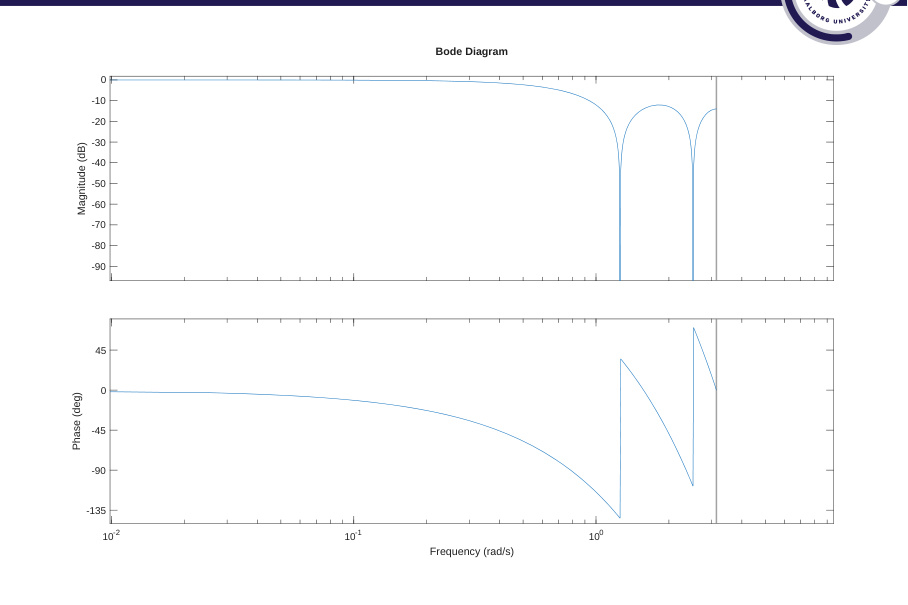
\includegraphics[width=\linewidth]{slide-30.jpg}
  \caption{Bode plot of the averaging filter: magnitude (top) and
           phase (bottom) vs.\ frequency.}
  \label{fig:slide30}
\end{figure}

The Bode plot shows both magnitude and phase response on a logarithmic
frequency axis. Key observations:

\begin{itemize}[leftmargin=1.5em]
  \item \textbf{Magnitude}: rolls off at higher frequencies, confirming
        the low-pass behaviour. The roll-off is not steep --- the
        averaging filter is a weak low-pass.
  \item \textbf{Phase}: introduces a frequency-dependent phase shift
        (delay). A constant-phase filter would delay all frequencies
        equally; the averaging filter does not, which means it distorts
        the shape of fast-changing signals.
\end{itemize}

\begin{keybox}
  \textbf{Key Takeaways --- averaging filter:}
  \begin{itemize}[leftmargin=1.5em, topsep=2pt]
    \item Simple to implement; just a running mean of the last $m$ samples.
    \item Works by convolution with a rectangular impulse response.
    \item Low-pass behaviour: smooths out high-frequency noise.
    \item Limitations: gradual roll-off, sidelobes, and phase distortion
          --- better filters exist for demanding applications.
    \item Larger $m$ = more smoothing but also more \textbf{lag}: because
          the output at time $k$ is the mean of the last $m$ samples, it
          is centred around $k - m/2$ --- the filter is always looking
          $m/2$ steps into the past. A real change in the signal only
          fully shows up in the output after $m$ new samples have been
          collected. More smoothing = older samples included = the output
          takes longer to catch up with reality.
  \end{itemize}
\end{keybox}

% ==============================================================================
%  TOPIC: Bessel and Butterworth Filters
% ==============================================================================
\section*{Slides 31--32 \quad Bessel and Butterworth Filters}

\subsection*{Filter Designs (Slide 31)}

Purpose-designed filters offer much better performance than the averaging
filter. The two most common choices for sensor applications are:

\textbf{Bessel filter:}
\begin{itemize}[leftmargin=1.5em]
  \item Designed for \textbf{maximally linear phase response} ---
        $d\varphi(\omega)/d\omega$ is as constant as possible.
  \item A constant phase slope means all frequencies are delayed by the
        same amount, so the \textbf{wave shape is preserved} in the
        passband. No distortion of the signal's time-domain structure.
  \item Harder to design directly in discrete time --- typically designed
        in continuous time and then discretised.
\end{itemize}

\textbf{Butterworth filter:}
\begin{itemize}[leftmargin=1.5em]
  \item Designed for \textbf{maximally flat magnitude} in the passband ---
        the gain is as close to 1 as possible across all passband
        frequencies.
  \item Steeper roll-off than Bessel at the cost of some phase non-linearity.
  \item Can be discretised directly using Tustin's method (bilinear
        transform), making it more straightforward to implement.
\end{itemize}

\begin{notebox}
  \textbf{Note --- Bessel vs Butterworth trade-off.}
  \begin{itemize}[leftmargin=1.5em, topsep=2pt]
    \item Need to preserve signal \emph{shape} (e.g.\ a step response or
          pulse)? $\to$ Bessel (linear phase).
    \item Need a flat passband and sharp roll-off? $\to$ Butterworth
          (flat magnitude).
  \end{itemize}
  Neither is universally better; the choice depends on whether timing
  or amplitude accuracy matters more.
\end{notebox}

\subsection*{Frequency Responses Compared (Slide 32)}

\begin{figure}[H]
  \centering
  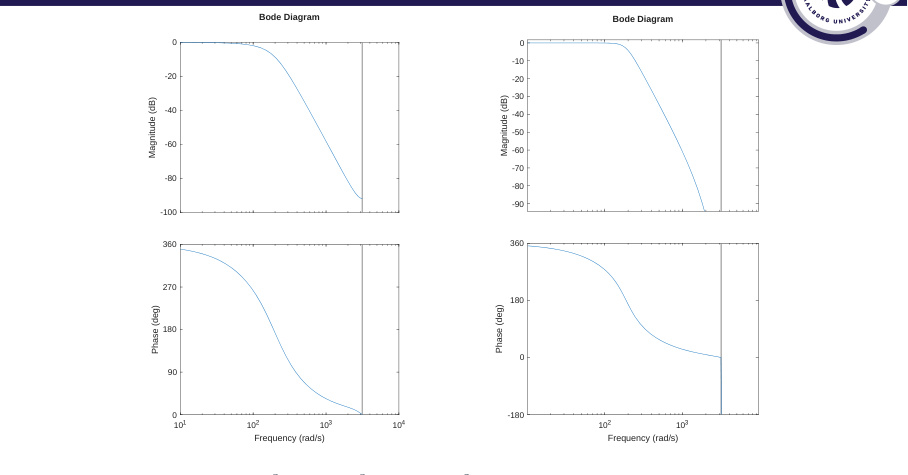
\includegraphics[width=\linewidth]{slide-32.jpg}
  \caption{Bode plots at cut-off 30\,Hz, sampling 1\,kHz.
           Left: Bessel. Right: Butterworth.}
  \label{fig:slide32}
\end{figure}

At the same cut-off frequency (30\,Hz) and sampling rate (1\,kHz) the
difference is visible in the Bode plots:
the Butterworth has a flatter passband and steeper roll-off, while the
Bessel has a more gradual roll-off but better-behaved phase.

The discrete-time transfer functions are:
\[
  F_\mathrm{Bes}(z) =
  \frac{10^{-3}(0.1814z^3 + 0.6253z^2 + 0.1351z)}
       {z^4 - 3.43z^3 + 4.431z^2 - 2.556z + 0.555}
\]
\[
  F_\mathrm{But}(z) =
  \frac{10^{-3}(0.06239z^4 + 0.2495z^3 + 0.3743z^2 + 0.2495z + 0.06239)}
       {z^4 - 3.508z^3 + 4.641z^2 - 2.743z + 0.6105}
\]

% ==============================================================================
%  TOPIC: Filter Implementation
% ==============================================================================
\section*{Slides 33--34 \quad Filter Implementation}

\subsection*{Difference Equation (Slide 33)}

\begin{figure}[H]
  \centering
  
\includegraphics[width=0.80\linewidth]{slide-33.jpg}
  \caption{Transfer function converted to a difference equation
           (numerator coefficients $b$, denominator $a$).}
  \label{fig:slide33}
\end{figure}

Any filter expressed as a rational $z$-domain transfer function:
\[
  \frac{\bar{Y}(z)}{Y(z)} =
  \frac{b_m z^m + b_{m-1}z^{m-1} + \cdots + b_0}
       {z^n + a_{n-1}z^{n-1} + \cdots + a_0}
\]
can be converted into a \textbf{difference equation} that is computed
recursively sample by sample:
\[
  \bar{y}_k = b_m y_k + b_{m-1}y_{k-1} + \cdots + b_0 y_{k-m}
              - a_{n-1}\bar{y}_{k-1} - \cdots - a_0\bar{y}_{k-n}
\]

Each new output $\bar{y}_k$ depends only on the current and past inputs
$y$ and past outputs $\bar{y}$ --- no convolution sum required, just
a short weighted sum updated every sample.

\begin{verbatim}
def filter(b, a, y):
    yfilt = np.zeros_like(y)
    for k in range(len(y)):
        s = 0.0
        for i in range(len(b)):
            if k - i > -1:
                s += b[i] * y[k - i]
        for i in range(1, len(a)):
            if k - i > -1:
                s -= a[i] * yfilt[k - i]
        yfilt[k] = s / a[0]
    return yfilt
\end{verbatim}

\begin{notebox}
  \textbf{Note --- IIR vs FIR.} A filter whose difference equation
  includes past \emph{output} terms ($\bar{y}_{k-i}$) is called
  \textbf{IIR} (Infinite Impulse Response) --- feedback makes its
  impulse response potentially infinite. The averaging filter has no
  feedback and is \textbf{FIR} (Finite Impulse Response).
  Bessel and Butterworth are IIR.
\end{notebox}

\subsection*{State Space Formulation (Slide 34)}

\begin{figure}[H]
  \centering
  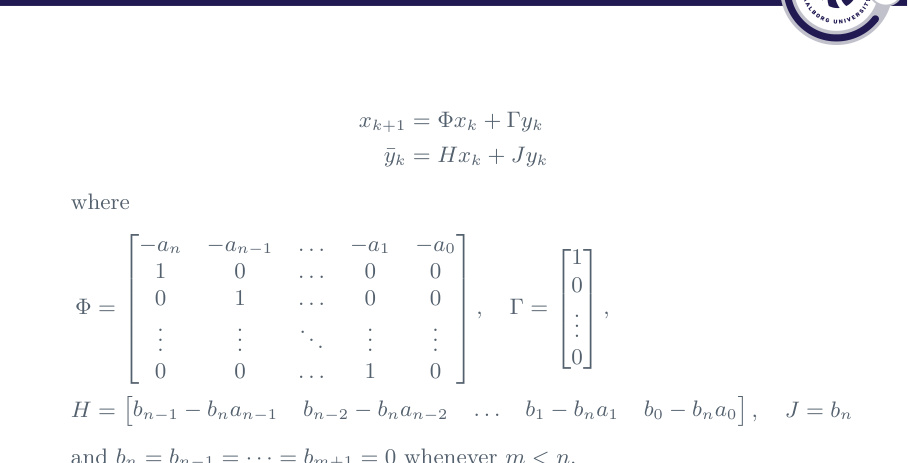
\includegraphics[width=\linewidth]{slide-34.jpg}
  \caption{State space matrices $\Phi$, $\Gamma$, $H$, $J$ for the
           discrete-time filter.}
  \label{fig:slide34}
\end{figure}

The same filter can be written in \textbf{state space form}:
\[
  x_{k+1} = \Phi x_k + \Gamma y_k
\]
\[
  \bar{y}_k = H x_k + J y_k
\]

This is structurally identical to the sensor model from slide 18, see \autoref{slide_18} ---
the filter is itself a discrete-time dynamical system, with $y_k$
(the noisy measurement) as its input and $\bar{y}_k$ (the filtered
output) as its output. The matrices $\Phi$, $\Gamma$, $H$, $J$ are
populated directly from the $a$ and $b$ coefficients of the transfer
function.

\begin{keybox}
  \textbf{Key Takeaway --- three equivalent representations:}
  \begin{itemize}[leftmargin=1.5em, topsep=2pt]
    \item \textbf{Convolution} --- intuitive, expensive for long filters.
    \item \textbf{Difference equation} --- efficient, easy to code
          sample-by-sample.
    \item \textbf{State space} --- most powerful; unifies filter and
          system model, enables Kalman filtering. Use linear algebra
          libraries in practice.
  \end{itemize}
\end{keybox}

% ==============================================================================
%  TOPIC: Filtering Performance
% ==============================================================================
\section*{Slide 35 \quad Filtering Performance}

\begin{figure}[H]
  \centering
  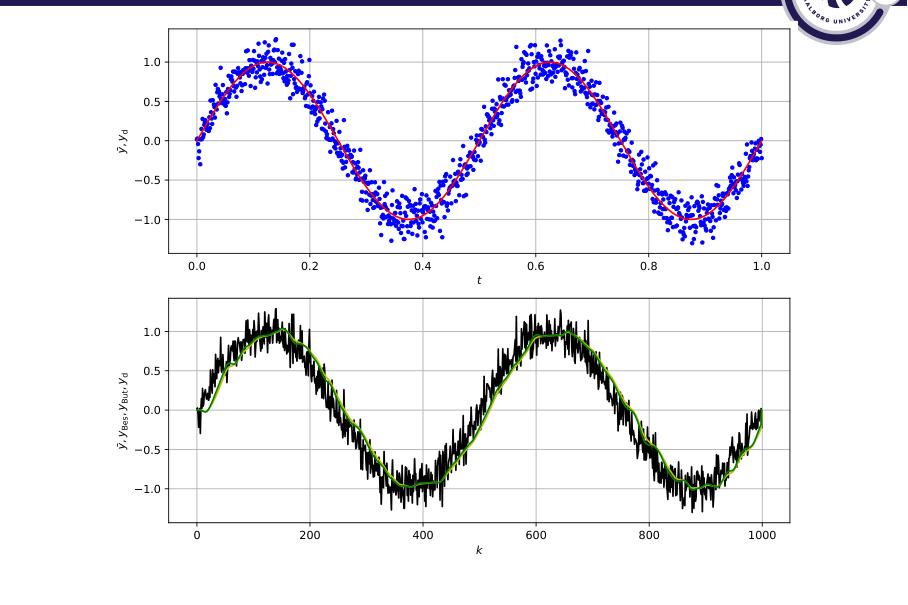
\includegraphics[width=0.95\linewidth]{slide-35.jpg}
  \caption{Top: continuous-time signal. Bottom: noisy discrete samples
           with Bessel (yellow) and Butterworth (green) filtered outputs
           vs.\ true deterministic signal (red).}
  \label{fig:slide35}
\end{figure}

The performance plot compares the two filters on a noisy sampled signal:

\begin{itemize}[leftmargin=1.5em]
  \item \textbf{Red} --- the true deterministic signal $y_d$
        (what we want to recover).
  \item \textbf{Yellow} --- Bessel filtered output. Follows the shape
        of the true signal faithfully with minimal phase distortion, but
        leaves slightly more noise through due to its gradual roll-off.
  \item \textbf{Green} --- Butterworth filtered output. Removes more
        noise (steeper roll-off) but introduces slightly more phase lag
        and shape distortion, visible at sharp transitions.
\end{itemize}

\begin{keybox}
  \textbf{Key Takeaway --- no free lunch.} Both filters reduce noise
  significantly compared to the raw signal. Butterworth suppresses more
  noise; Bessel preserves shape better. The ``right'' choice depends on
  whether the application is more sensitive to noise amplitude or to
  signal timing and shape.
\end{keybox}

% ==============================================================================
%  TOPIC: Summary
% ==============================================================================
\section*{Slide 36 \quad Lecture Summary}

The lecture covered three broad areas:

\textbf{Simple sensors:} A sensor is ``simple'' if it measures one
continuous physical quantity, provides a straightforward analog or
digital interface, and requires no extensive processing. Examples
covered: Hall effect (magnetic field), NTC thermistor (temperature),
DHT11 (temperature + humidity).

\textbf{Noise:}
\begin{itemize}[leftmargin=1.5em]
  \item \textbf{Gaussian / white noise} --- normally distributed,
        equal power at all frequencies, zero autocorrelation for
        $\kappa \neq 0$. The standard model for measurement noise.
  \item \textbf{Coloured noise} --- unequal power across frequencies,
        but still uncorrelated with time-shifted versions of itself.
        Pink and red noise have more low-frequency power; blue and
        violet have more high-frequency power.
\end{itemize}

\textbf{Filtering --- why low-pass filters remove noise:}
The key insight is in the frequency domain. The true signal $y_{d,k}$
is typically \textbf{slowly varying} --- its energy is concentrated at
\emph{low} frequencies. Measurement noise $\nu_k$ is i.i.d.\
(independent and identically distributed), which means each sample is
independent of every other --- there is no correlation between adjacent
samples. This is exactly the definition of \textbf{white noise}: flat
power spectral density, equal energy at \emph{all} frequencies,
including the high ones.

A \textbf{low-pass filter} passes low frequencies and attenuates high
frequencies. Since the signal lives at low frequencies and the noise is
spread across all frequencies, the filter preferentially keeps the signal
and cuts the noise:

\begin{center}
\small
\begin{tabular}{lll}
  \textbf{Component} & \textbf{Frequency content} & \textbf{After low-pass} \\
  \hline
  True signal $y_{d,k}$ & concentrated at low $f$ & passes through \\
  i.i.d.\ noise $\nu_k$ & spread across all $f$ equally & high-$f$ portion cut \\
\end{tabular}
\end{center}

The more i.i.d.\ (white) the noise, the more evenly spread it is, and
the more of it a low-pass filter removes. This is why assuming white
Gaussian noise is both convenient and practically effective.

Bessel and Butterworth are both low-pass filters with a sharper,
better-controlled cut-off than the averaging filter --- Butterworth
maximises how flat the passband is (signal distortion minimised),
Bessel maximises phase linearity (shape of the signal preserved).
Three implementations (convolution, difference equation, state space)
are equivalent descriptions of the same filter.

\begin{keybox}
  \textbf{Overall Key Takeaway:} Every real sensor measurement is
  $y_k = y_{d,k} + \nu_k$. The sensor determines $y_{d,k}$; the noise
  model describes $\nu_k$; the filter recovers the best estimate of
  $y_{d,k}$ from the corrupted $y_k$. These three elements --- sensor,
  noise model, filter --- form the complete picture of a simple sensor
  system.
\end{keybox}

\end{document}
